\documentclass[12pt,a4paper]{article}
\usepackage[UTF8]{ctex}
\usepackage{geometry}
\usepackage{graphicx}
\usepackage{float}
\usepackage{amsmath}
\usepackage{amsfonts}
\usepackage{amssymb}
\usepackage{booktabs}
\usepackage{multirow}
\usepackage{array}
\usepackage{longtable}
\usepackage{enumerate}
\usepackage{fancyhdr}
\usepackage{lastpage}
\usepackage{hyperref}
\usepackage{siunitx}
\usepackage{enumitem}

% 页面设置
\geometry{left=2.5cm,right=2.5cm,top=2.5cm,bottom=2.5cm}

% 行距设置
\linespread{1.2}

% 段落缩进
\setlength{\parindent}{2em}

% 修复页眉高度问题
\setlength{\headheight}{14.49998pt}
\addtolength{\topmargin}{-2.49998pt}

% 页眉页脚设置
\pagestyle{fancy}
\fancyhf{}
\fancyhead[C]{实\hspace{0.5em}验\hspace{0.5em}报\hspace{0.5em}告}
\fancyfoot[C]{\thepage}

\begin{document}

% 正文第一行标题
\noindent
{\Large \textbf{实验九：}\underline{\textbf{一阶电路的响应}}} \hfill {\Large \textbf{实验成绩：}\underline{\hspace{3cm}}}
\vspace{0.5cm}

\section*{一、实验目的}
\begin{enumerate}
    \item 学习用示波器观察一阶电路的过渡过程。
    \item 学习用示波器测量一阶电路时间常数的方法。
    \item 观察一阶电路阶跃响应和方波激励响应的规律和特点。
\end{enumerate}

\section*{二、实验原理}

\begin{enumerate}
    \item 可以用一阶微分方程描述的含有储能元件的动态电路称为一阶电路。
    
    \item 电路的过渡过程可以分为零输入响应、零状态响应和全响应。
    
    对于一阶RC电路的电容电压$u_c$响应表达式为：$u_c(t) = u_c(0^+)e^{-\frac{t}{\tau}} + V_s(1-e^{-\frac{t}{\tau}})$
    
    其中：$u_c(0^+)$为电容初始电压；$V_s$为外加直流激励；$\tau = RC$为时间常数。
    
    当$V_s = 0$时为零输入响应；当$u_c(0^+) = 0$时为零状态响应；当$u_c(0^+) \neq 0$且$V_s \neq 0$时为全响应（零输入响应与零状态响应的叠加）。
    
    \item 阶跃响应
    
    当外加激励为阶跃信号时，电路的零状态响应称为阶跃响应。
    
    一阶RC电路对方波脉冲序列的响应可以看作是多个阶跃响应的叠加。
    
    \item 时间常数及测量
    
    对于充电曲线，当电压上升到稳态值的63.2\%时，对应的时间即为一个时间常数$\tau$；
    
    对于放电曲线，当电压下降到初始值的36.8\%时，对应的时间为一个时间常数$\tau$。
    
    可通过示波器测定电压变化到稳态值的63.2\%或下降到初始值的36.8\%所对应的时间来确定时间常数。
\end{enumerate}

\section*{三、思考题}
\begin{enumerate}
    \item 若用示波器观察一阶RC电路中电阻上的电压波形，应如何连接？
    
    \textbf{解：}要观察电阻上的电压波形，应将示波器探头连接在电阻两端：
    \begin{itemize}
        \item 将示波器通道的探头（红色）连接到电阻的一端
        \item 将示波器的接地端（黑色）连接到电阻的另一端
        \item 注意：示波器的接地端应与电路的参考地保持一致
        \item 如果需要同时观察多个元件的电压，可以使用多个通道，但所有通道的接地端必须共地
    \end{itemize}
    \vspace{0.5cm}
    
    \item 在RC串联电路中，如果电路的时间常数$\tau = 0.04$s，为完整显示波形，示波器的水平扫描速度应不小于多少？
    
    \textbf{解：}为完整显示一阶电路的过渡过程，通常需要观察$(3\sim5)\tau$的时间范围。
    \begin{itemize}
        \item 取$5\tau$作为完整显示时间：$T_{display} = 5\tau = 5 \times 0.04 = 0.2$s
        \item 示波器屏幕一般有10个水平格，要在一屏内显示完整波形
        \item 水平扫描速度应为：$\frac{0.2\text{s}}{10} = 0.02$s/div = 20 ms/div
        \item 因此，示波器的水平扫描速度应不大于20 ms/div（或更快的扫描速度）
    \end{itemize}
    \vspace{0.5cm}

    \item 现想提高一阶RC电路中电阻电压的最大值，若保持电源和电容参数不变，仅通过提升电阻值以增大分压，是否可行？
    
    \textbf{解：}不可行。
    \begin{itemize}
        \item 在RC串联电路中，对于直流稳态：电容相当于开路，电阻上的电压等于电源电压，与电阻阻值无关
        \item 对于交流信号：电阻电压幅值为$U_R = U_s \cdot \frac{R}{\sqrt{R^2 + (\frac{1}{\omega C})^2}}$
        \item 当$R$增大时，虽然分子增大，但分母增大得更快（当$R \ll \frac{1}{\omega C}$时）
        \item 当$R \gg \frac{1}{\omega C}$时，$U_R \approx U_s$，继续增大$R$无法提高$U_R$
        \item 因此，单纯提高电阻值并不能有效提高电阻电压的最大值
    \end{itemize}
    \vspace{0.5cm}
    
    \item 增大一阶RC电路中电容的容值，对电路电流及电阻电压有何影响？
    
    \textbf{解：}增大电容容值会产生以下影响：
    \begin{itemize}
        \item \textbf{对时间常数的影响：}$\tau = RC$增大，电路响应变慢
        \item \textbf{对电流的影响：}
        \begin{itemize}
            \item 瞬态过程中，充放电电流峰值不变（$I_0 = \frac{U_s}{R}$）
            \item 但电流衰减速度变慢，电流持续时间更长
            \item 对于交流信号，容抗$X_C = \frac{1}{\omega C}$减小，电流幅值增大
        \end{itemize}
        \item \textbf{对电阻电压的影响：}
        \begin{itemize}
            \item 瞬态过程中，电阻电压初始值不变，但衰减速度变慢
            \item 对于交流信号，电阻电压幅值增大（容抗减小，电流增大）
            \item 电容电压与电源电压的相位差减小
        \end{itemize}
    \end{itemize}
    \vspace{0.5cm}
    
    \item 已知一阶RC电路中，电阻$R = \SI{30}{\kilo\ohm}$，电容$C = \SI{0.01}{\micro\farad}$，请计算时间常数$\tau$，并结合其物理意义，拟定测量$\tau$的方案，简要描述测量步骤。
    
    \textbf{解：}
    
    \textbf{(1) 计算时间常数：}
    \begin{align*}
        \tau &= RC = 30 \times 10^3 \times 0.01 \times 10^{-6} \\
        &= 30 \times 10^3 \times 10^{-8} \\
        &= 3 \times 10^{-4} \text{ s} = 0.3 \text{ ms}
    \end{align*}
    
    \textbf{(2) 物理意义：}时间常数$\tau$表征了一阶电路过渡过程的快慢。在充电过程中，经过时间$\tau$后，电容电压上升到稳态值的63.2\%；在放电过程中，经过时间$\tau$后，电容电压下降到初始值的36.8\%。
    
    \textbf{(3) 测量方案：}
    \begin{enumerate}
        \item \textbf{方法一：充电曲线法}
        \begin{itemize}
            \item 用方波信号作为激励源（频率应满足$T \gg 5\tau$，建议$f \approx 100$ Hz）
            \item 示波器CH1接信号源，CH2接电容两端
            \item 调节示波器使充电曲线完整显示
            \item 测量稳态电压$U_{max}$，计算$0.632 U_{max}$对应的电压值
            \item 使用光标功能测量从充电开始到电压达到$0.632 U_{max}$所需的时间，即为$\tau$
        \end{itemize}
        \item \textbf{方法二：放电曲线法}
        \begin{itemize}
            \item 电路连接同上
            \item 观察放电曲线
            \item 测量初始电压$U_0$，计算$0.368 U_0$对应的电压值
            \item 测量从放电开始到电压降至$0.368 U_0$所需的时间，即为$\tau$
        \end{itemize}
        \item \textbf{方法三：多点测量法}
        \begin{itemize}
            \item 测量充电或放电曲线上多个点的时间和电压值
            \item 利用$u_C(t) = U(1-e^{-t/\tau})$或$u_C(t) = Ue^{-t/\tau}$拟合曲线
            \item 通过数据拟合得到$\tau$值
        \end{itemize}
    \end{enumerate}
\end{enumerate}

\section*{四、实验任务与线路}
\begin{enumerate}
    \item 研究 RC 电路在正弦波 $u_s$ 激励电源作用下的电容电压和电流响应。实验电路如下图所示，分别描绘出 $5RC = T/2$、$5RC \ll T/2$ 和 $5RC \gg T/2$ 下，$u_s(t)$、$u_C(t)$ 和 $i_C(t)$ 的波形。（正弦波激励电压源的参数：$u_{s-p} = 10\text{V}$，$f = 1\text{kHz}$；$C = 0.1\mu\text{F}$） 
    \begin{figure}[H]
    \centering
    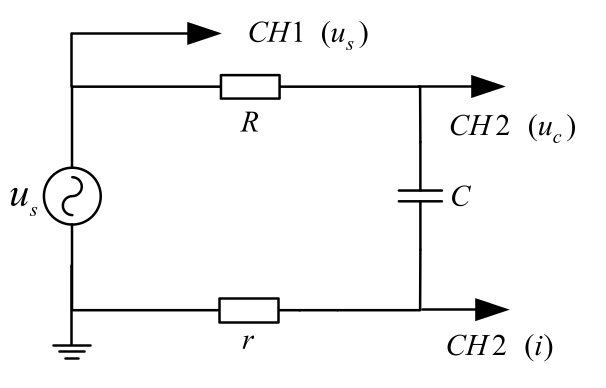
\includegraphics[width=0.8\textwidth]{templete_preview/1.png}
    \caption{实验线路图}
    \label{fig:circuit}
\end{figure}
\end{enumerate}

\section*{五、实验数据记录与分析}
\subsection*{1. 5RC = T/2条件下的波形记录}
\begin{figure}[H]
\centering
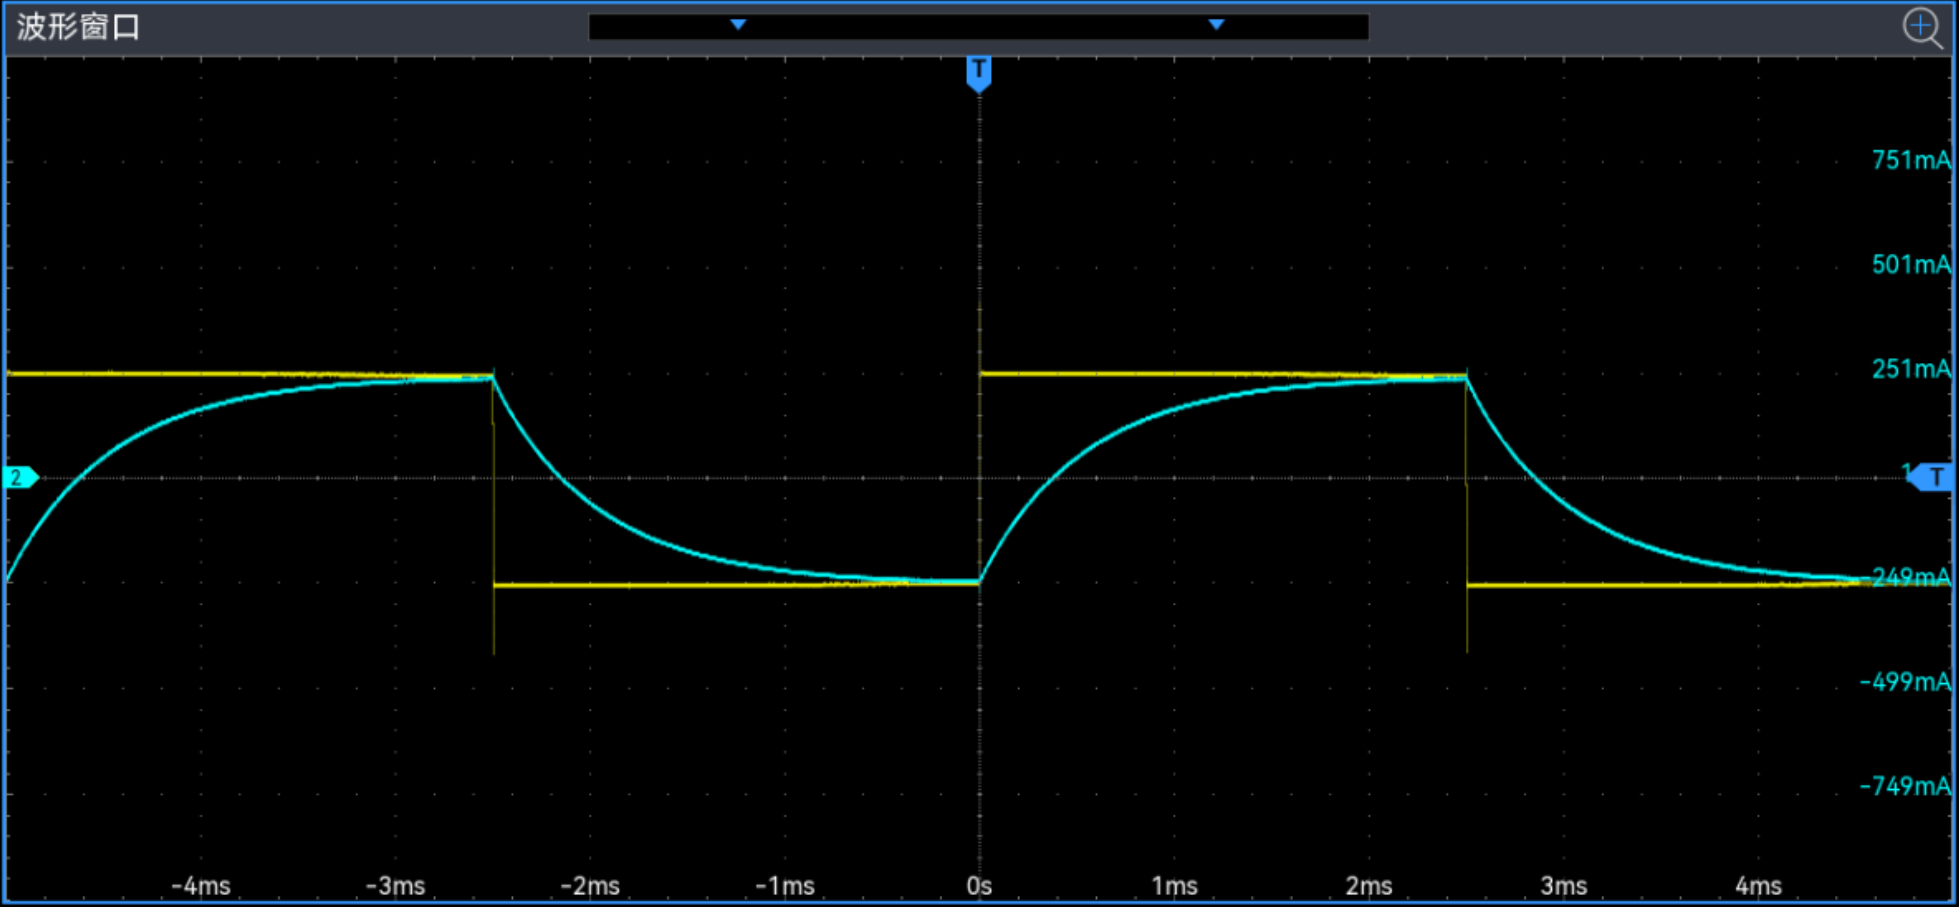
\includegraphics[width=0.8\textwidth]{E9_picture/1_5000omega.png}
\caption{5RC = T/2条件下的波形}
\label{fig:waveform1}
\end{figure}

\textbf{数据分析：}
\begin{itemize}[label={}]
    \item 当$ R = 5k\Omega$时，满足条件 $5RC = T/2$，电压，电流刚好达到峰值。
\end{itemize}

\subsection*{2. 5RC $\ll$ T/2条件下的波形记录}
\begin{figure}[H]
\centering
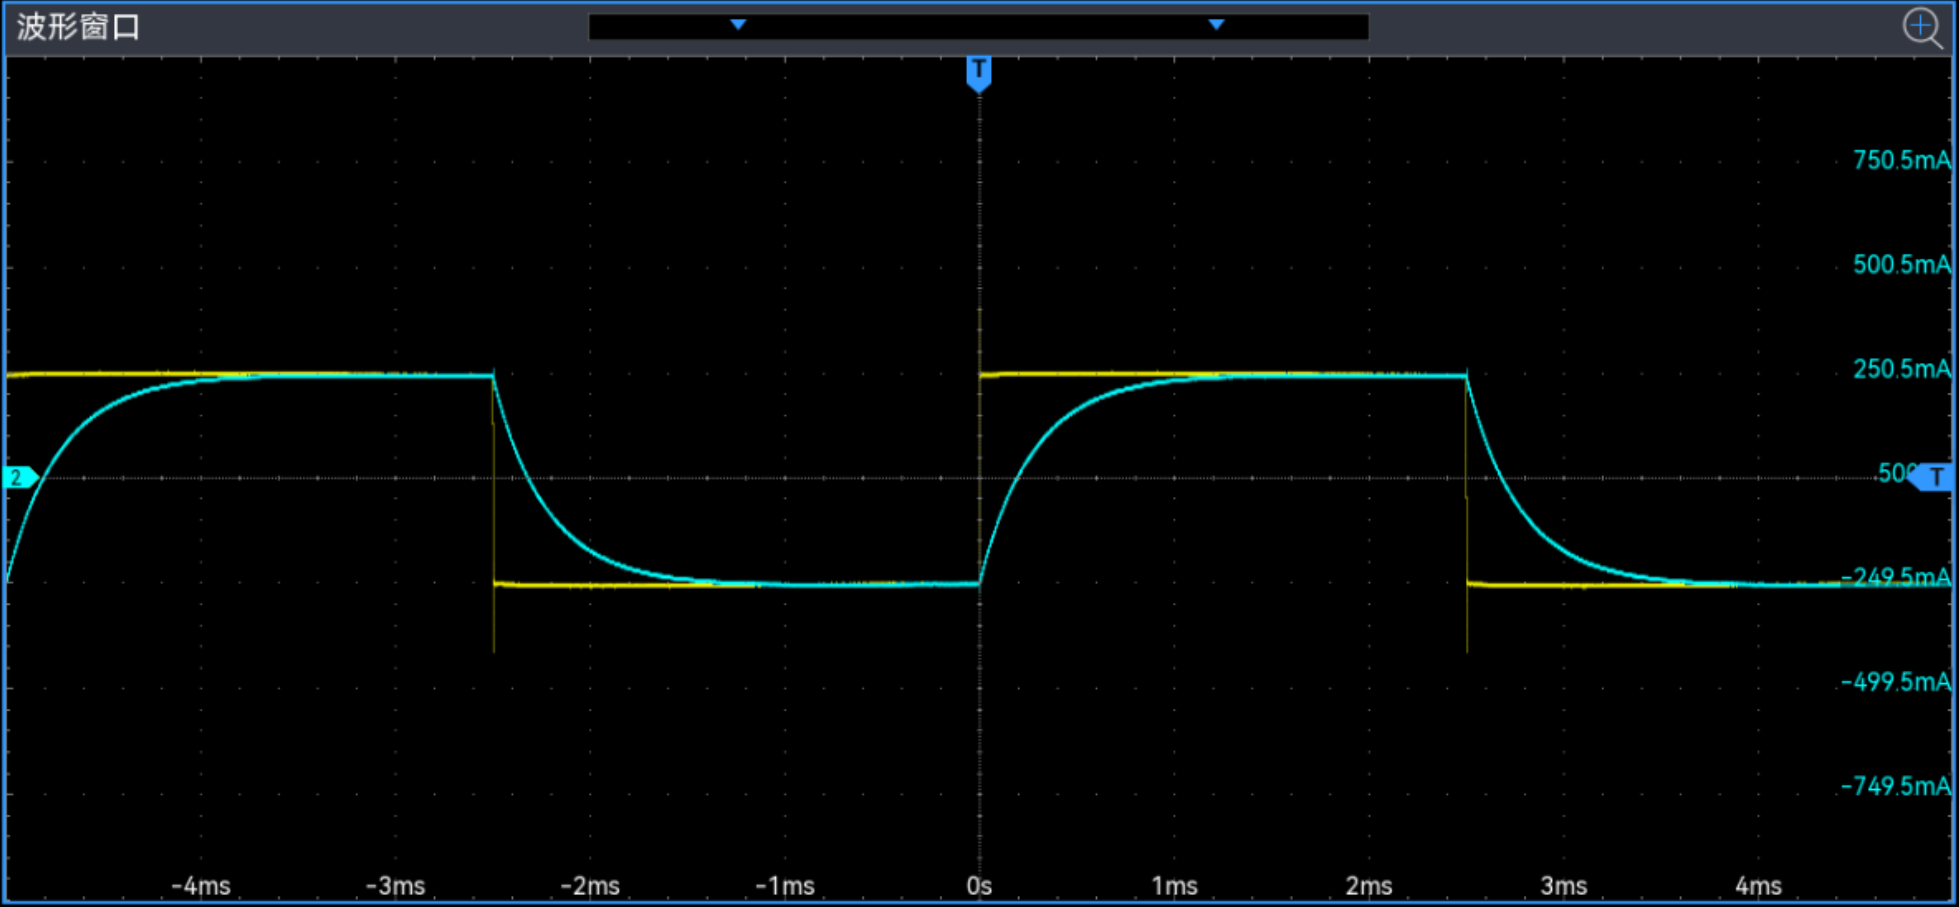
\includegraphics[width=0.8\textwidth]{E9_picture/1_2500omega.png}
\caption{5RC $\ll$ T/2条件下的波形}
\label{fig:waveform2}
\end{figure}

\textbf{数据分析：}
\begin{itemize}[label={}]
    \item 当$ R = 2.5k\Omega$时，满足条件 $5RC \ll T/2$，时间充足，电压、电流很早便能达到峰值。
\end{itemize}

\subsection*{3. 5RC $\gg$ T/2条件下的波形记录}
\begin{figure}[H]
\centering
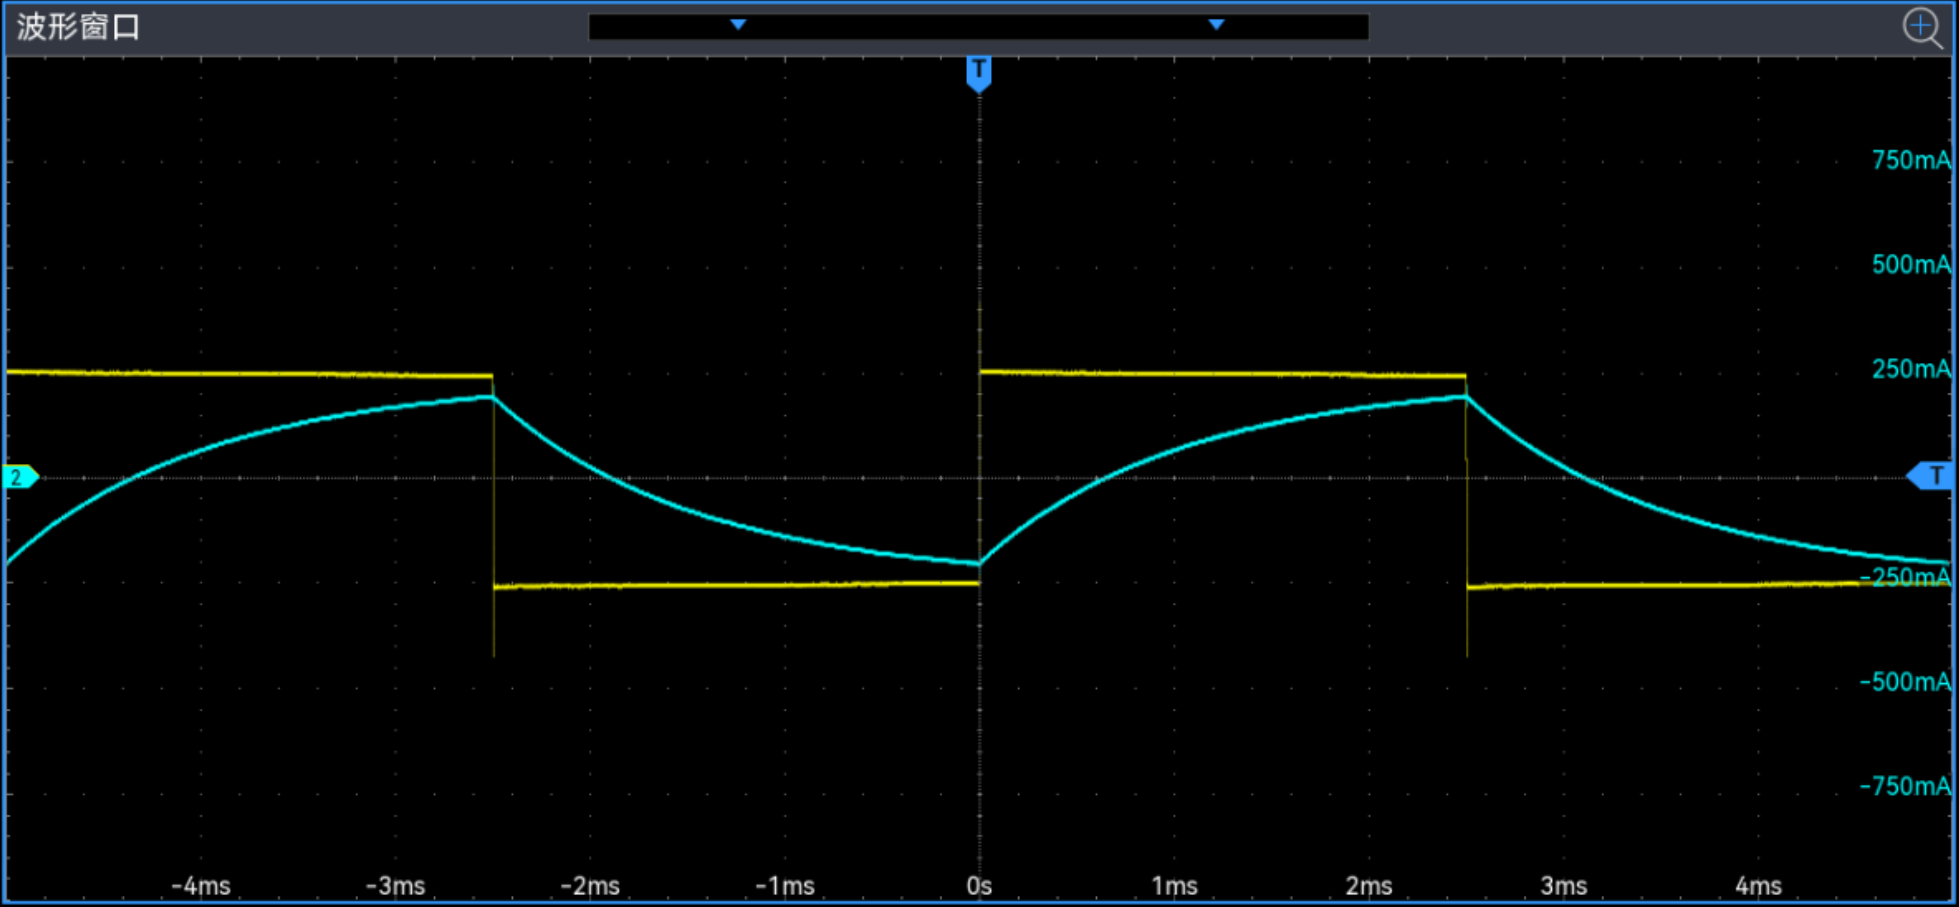
\includegraphics[width=0.8\textwidth]{E9_picture/1_10000omega.png}
\caption{5RC $\gg$ T/2条件下的波形}
\label{fig:waveform3}
\end{figure}

\textbf{数据分析：}
\begin{itemize}[label={}]
    \item 当$ R = 10k\Omega$时，满足条件 $5RC \gg T/2$，电压、电流回复不充分，$\tau$过大 ，导致无法达到峰值，只能周期反复。
\end{itemize}

\section*{六、实验小结}
通过本次实验，我利用示波器观察和分析了一阶RC电路的过渡过程和稳态响应，深入了解了一阶电路的响应特性和规律。实验中，我掌握了示波器的噪声滤波和平均功能的使用方法，有效地消除了信号中的毛刺和干扰，获得了清晰的波形数据。

实验使我对一阶电路的时间常数测量方法有了深刻的理解，学会了通过观察电压上升到稳态值63.2\%或下降到初始值36.8\%的时间来确定时间常数。同时，通过对不同参数条件下电路响应的对比分析，加深了对一阶电路动态特性的认识。

\end{document}